% 12 variables in here:
% u_1 = 0.0, h_1 = 10.0, U_1 = 0.0, H_1 = 10.0, u_2 = -1.0, h_2 = 10.0, U_2 = 0.0, H_2 = 10.0, u_3 = 0.0, h_3 = 10.0, U_3 = 0.0, H_3 = 10.0
\begin{figure}[h!t]
  \centering
  % \subfigure[Height for points $p_1^L$ and $p_3^L$ (same for $p_1^R$ and $p_3^R$ respectively).] {
  % \begin{tikzpicture}
  %   \node at (0,0) {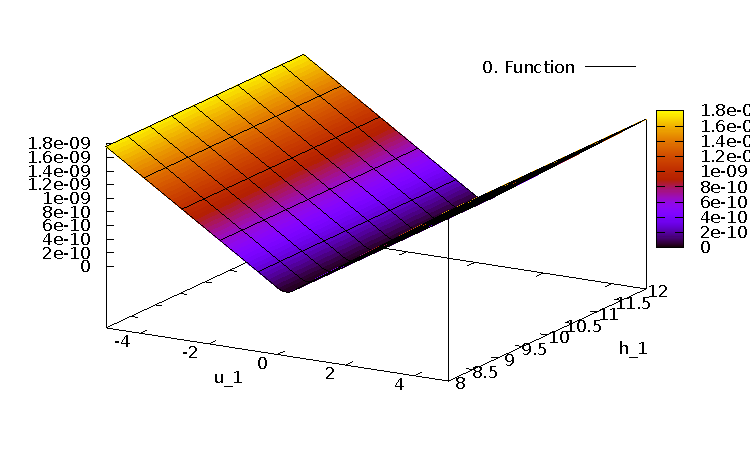
\includegraphics[scale=\zoomfactor]{{{3_punkte_2_impuls_verringert/x_y_0.0_10.0_-1.0_10.0_0.0_10.0_0.0_10.0_0.0_10.0f0}}}  };
  %   \fill[white] (.8,1.2) rectangle (1.75,1.5);
  %   \node[align=right, text width=3cm] at (.2,1.33) {\textsf{\tiny{Height error}}};
  % \end{tikzpicture}
  % \begin{tikzpicture}
  %   \node at (0,0) {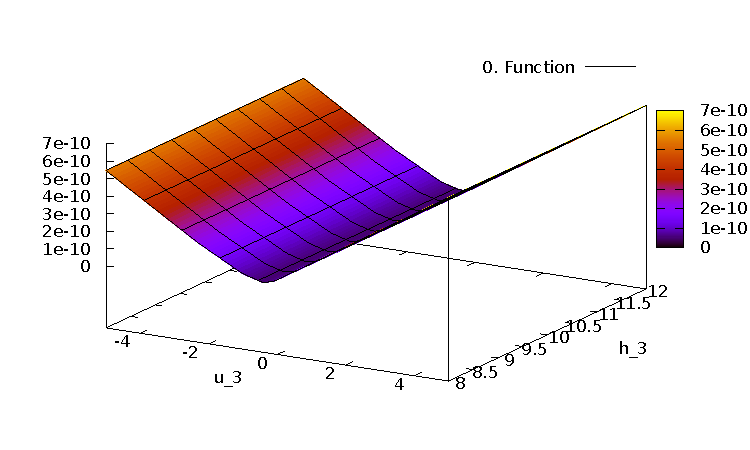
\includegraphics[scale=\zoomfactor]{{{3_punkte_2_impuls_verringert/0.0_10.0_0.0_10.0_-1.0_10.0_0.0_10.0_x_y_0.0_10.0f0}}}  };
  %   \fill[white] (.8,1.2) rectangle (1.75,1.5);
  %   \node[align=right, text width=3cm] at (.2,1.33) {\textsf{\tiny{Height error}}};
  % \end{tikzpicture}
  % % 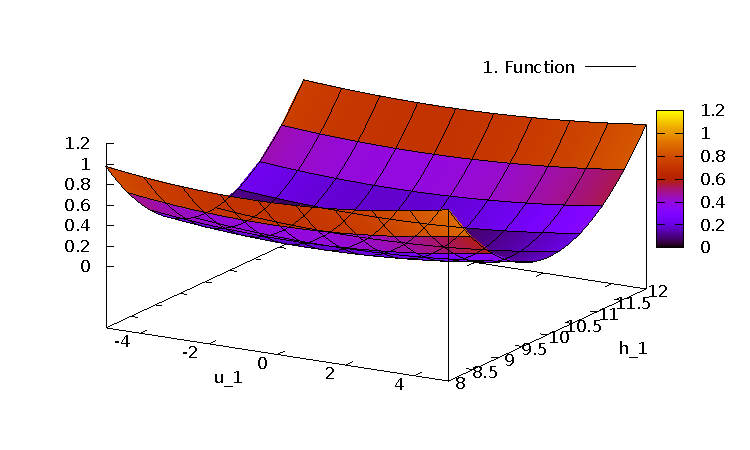
\includegraphics[scale=\zoomfactor]{{{3_punkte_2_impuls_verringert/x_y_0.0_10.0_-1.0_10.0_0.0_10.0_0.0_10.0_0.0_10.0f1}}}  
  % }
  %   \subfigure[Height for points $p_2^L$ and $p_2^R$. Slight difference in scale.] {
  %   \begin{tikzpicture}
  %     \node at (0,0) {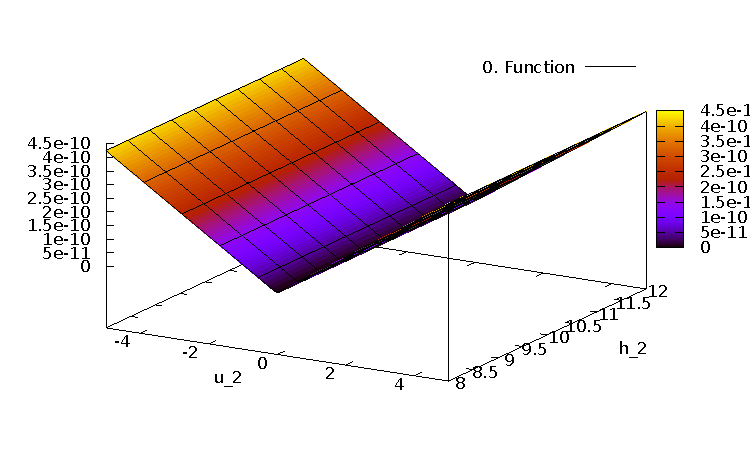
\includegraphics[scale=\zoomfactor]{{{3_punkte_2_impuls_verringert/0.0_10.0_0.0_10.0_x_y_0.0_10.0_0.0_10.0_0.0_10.0f0}}}  };
  %     \fill[white] (.8,1.2) rectangle (1.75,1.5);
  %     \node[align=right, text width=3cm] at (.2,1.33) {\textsf{\tiny{Height error}}};
  %   \end{tikzpicture}
  %   \begin{tikzpicture}
  %     \node at (0,0) {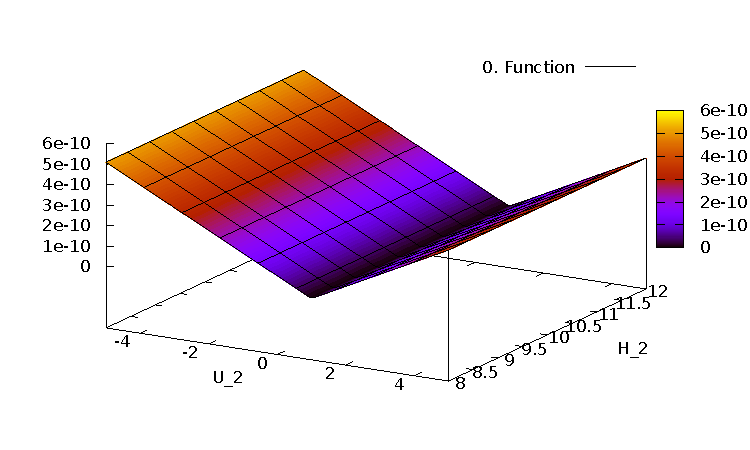
\includegraphics[scale=\zoomfactor]{{{3_punkte_2_impuls_verringert/0.0_10.0_0.0_10.0_-1.0_10.0_x_y_0.0_10.0_0.0_10.0f0}}}  };
  %     \fill[white] (.8,1.2) rectangle (1.75,1.5);
  %     \node[align=right, text width=3cm] at (.2,1.33) {\textsf{\tiny{Height error}}};
  %   \end{tikzpicture}
  % %   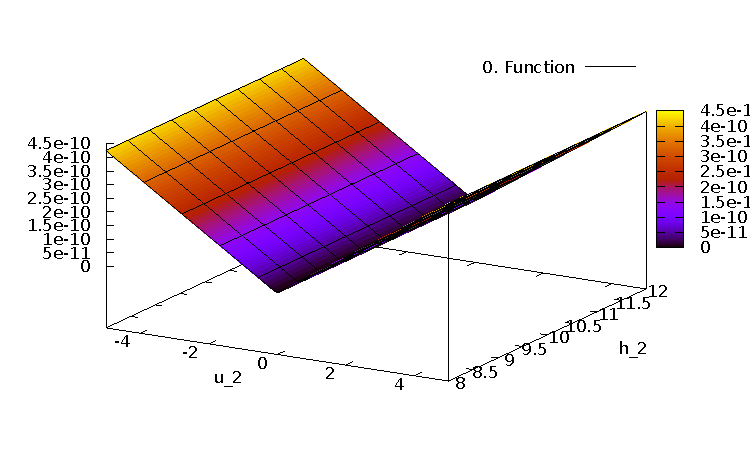
\includegraphics[scale=\zoomfactor]{{{3_punkte_2_impuls_verringert/0.0_10.0_0.0_10.0_x_y_0.0_10.0_0.0_10.0_0.0_10.0f0}}}  
  % %   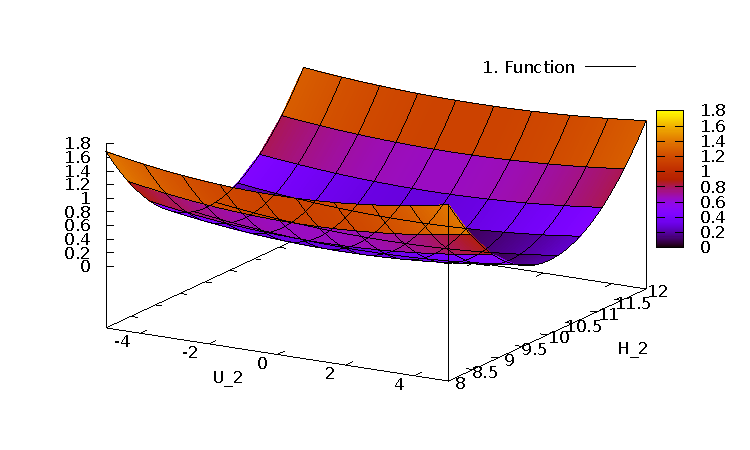
\includegraphics[scale=\zoomfactor]{{{3_punkte_2_impuls_verringert/0.0_10.0_0.0_10.0_0.0_10.0_x_y_0.0_10.0_0.0_10.0f1}}}  
  % }
  \subfigure[Momentum for points $p_1^L$ resp. $p_3^L$] {
    \begin{tikzpicture}
      \node at (0,0) {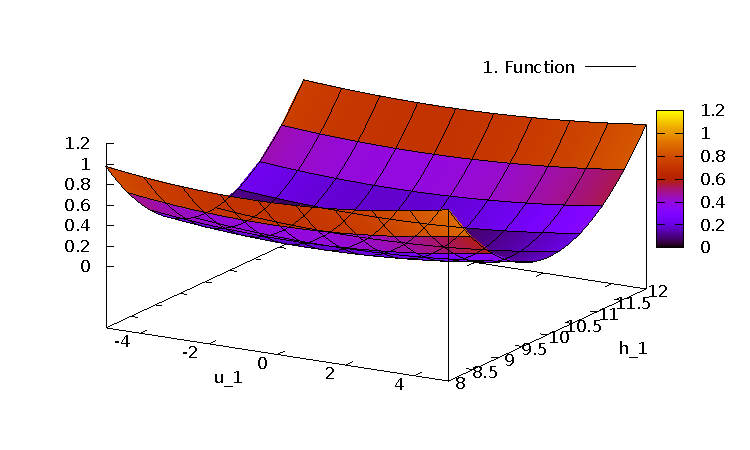
\includegraphics[scale=\zoomfactor]{{{3_punkte_2_impuls_verringert/x_y_0.0_10.0_-1.0_10.0_0.0_10.0_0.0_10.0_0.0_10.0f1}}}  };
      \fill[white] (.8,1.2) rectangle (1.75,1.5);
      \node[align=right, text width=3cm] at (.2,1.33) {\textsf{\tiny{Momentum error}}};
    \end{tikzpicture}
  }
  \subfigure[Momentum for points $p_2^L$]{
    \begin{tikzpicture}
      \node at (0,0) {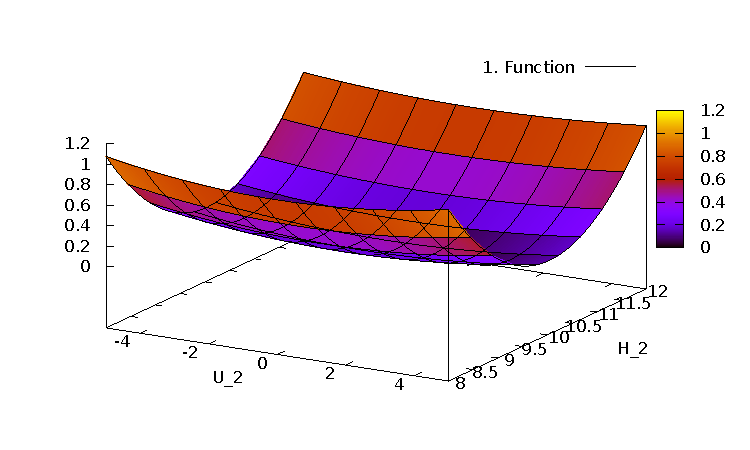
\includegraphics[scale=\zoomfactor]{{{3_punkte_2_impuls_verringert/0.0_10.0_0.0_10.0_-1.0_10.0_x_y_0.0_10.0_0.0_10.0f1}}}  };
      \fill[white] (.8,1.2) rectangle (1.75,1.5);
      \node[align=right, text width=3cm] at (.2,1.33) {\textsf{\tiny{Momentum error}}};
    \end{tikzpicture}
    % 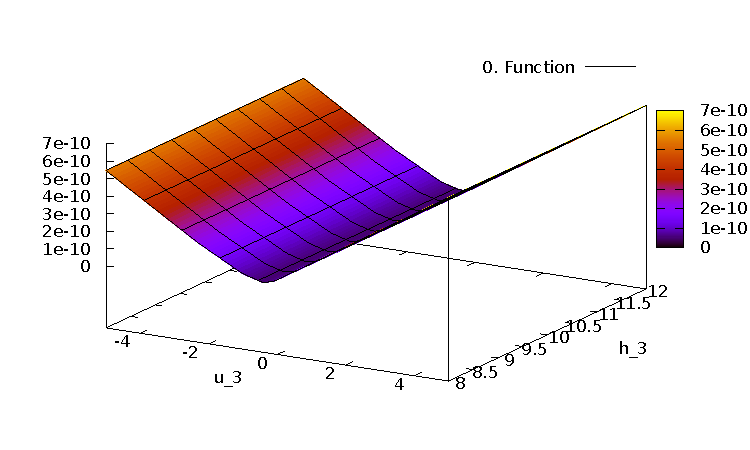
\includegraphics[scale=\zoomfactor]{{{3_punkte_2_impuls_verringert/0.0_10.0_0.0_10.0_-1.0_10.0_0.0_10.0_x_y_0.0_10.0f0}}}  
    % 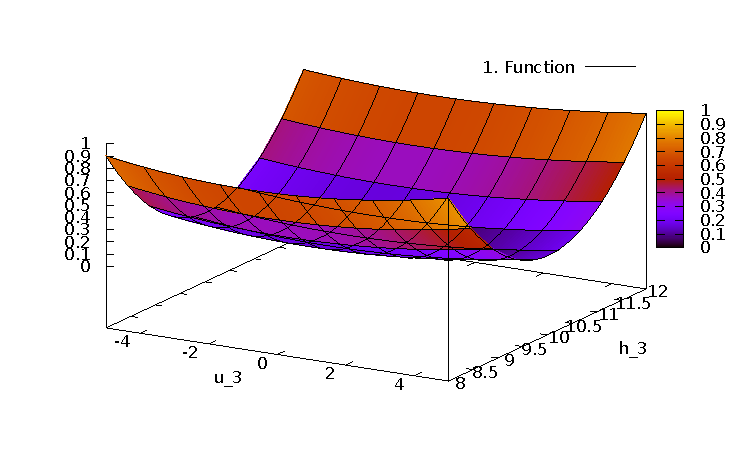
\includegraphics[scale=\zoomfactor]{{{3_punkte_2_impuls_verringert/0.0_10.0_0.0_10.0_-1.0_10.0_0.0_10.0_x_y_0.0_10.0f1}}}  
  }

  % \subfigure[Height and momentum for point $P_1$] {
  % 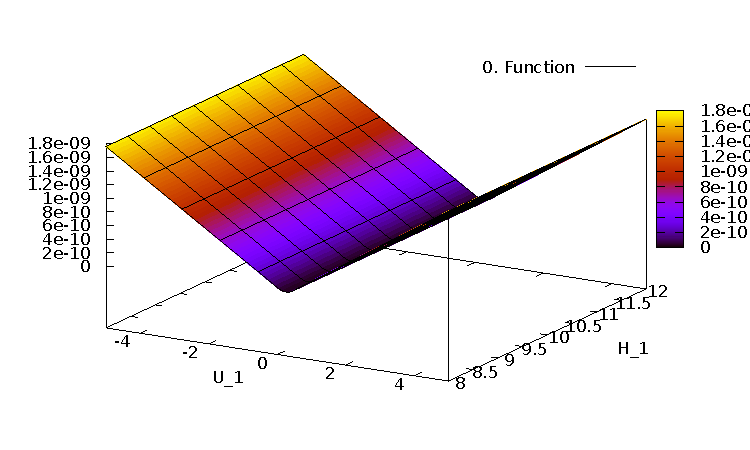
\includegraphics[scale=\zoomfactor]{{{3_punkte_2_impuls_verringert/0.0_10.0_x_y_-1.0_10.0_0.0_10.0_0.0_10.0_0.0_10.0f0}}}  
  % 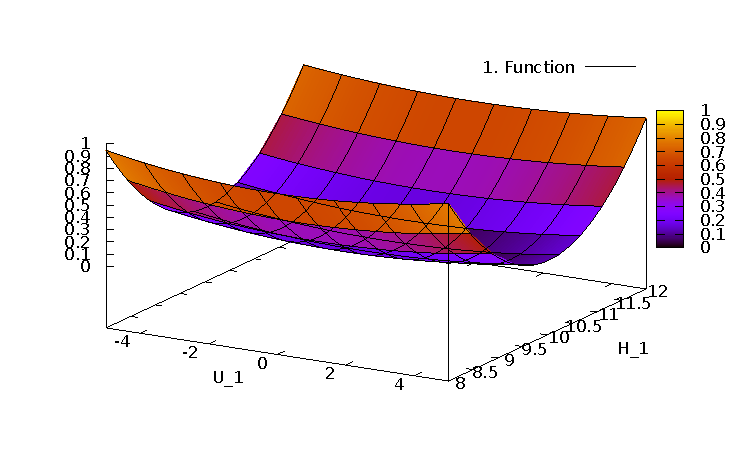
\includegraphics[scale=\zoomfactor]{{{3_punkte_2_impuls_verringert/0.0_10.0_x_y_-1.0_10.0_0.0_10.0_0.0_10.0_0.0_10.0f1}}}  
  % }

  %   \subfigure[Height and momentum for point $P_2$] {
  %   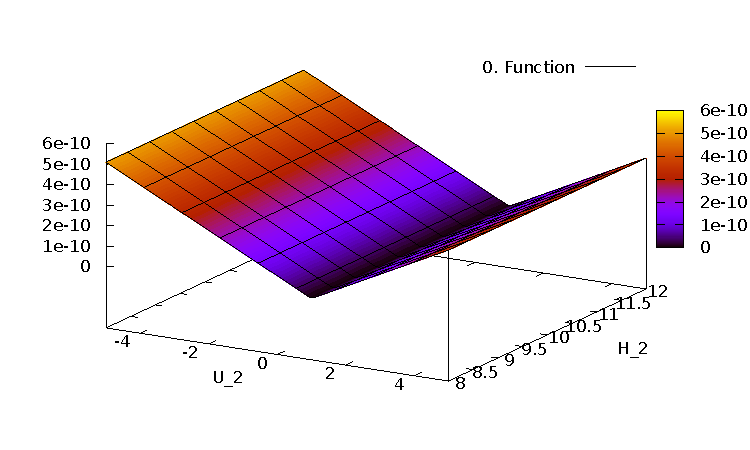
\includegraphics[scale=\zoomfactor]{{{3_punkte_2_impuls_verringert/0.0_10.0_0.0_10.0_-1.0_10.0_x_y_0.0_10.0_0.0_10.0f0}}}  
  %   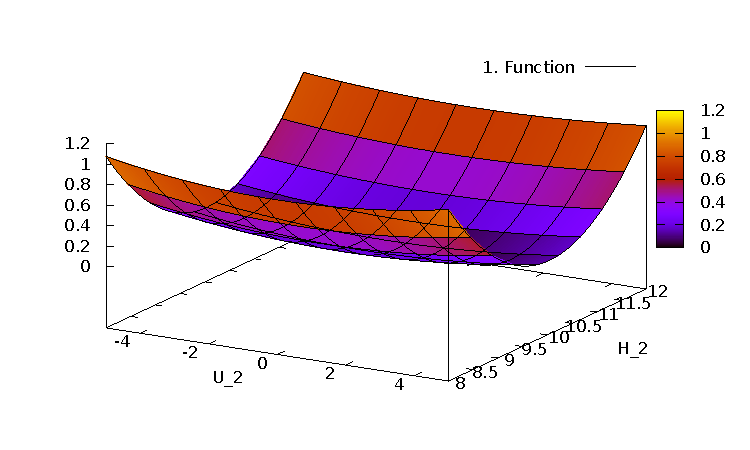
\includegraphics[scale=\zoomfactor]{{{3_punkte_2_impuls_verringert/0.0_10.0_0.0_10.0_-1.0_10.0_x_y_0.0_10.0_0.0_10.0f1}}}  
  % }

  %   \subfigure[Height and momentum for point $P_3$] {
  %   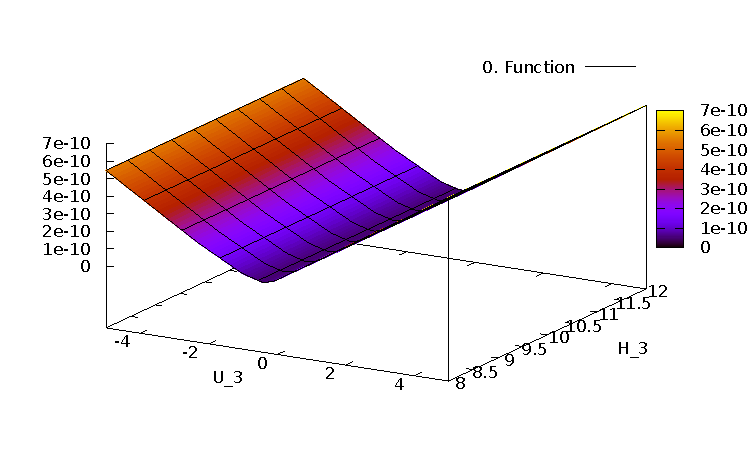
\includegraphics[scale=\zoomfactor]{{{3_punkte_2_impuls_verringert/0.0_10.0_0.0_10.0_-1.0_10.0_0.0_10.0_0.0_10.0_x_yf0}}}  
  %   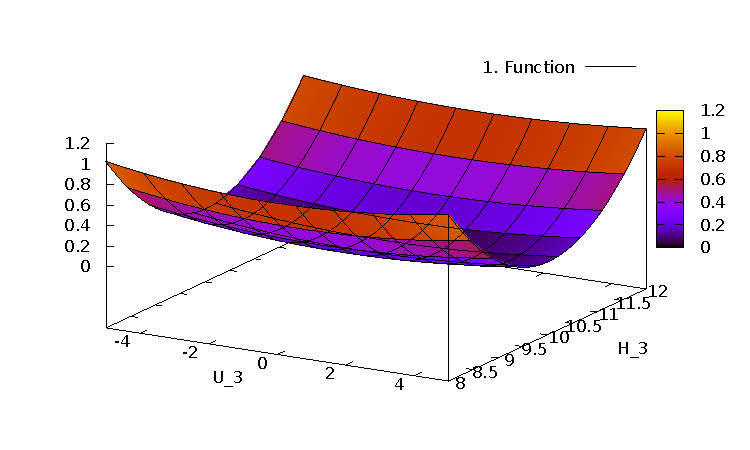
\includegraphics[scale=\zoomfactor]{{{3_punkte_2_impuls_verringert/0.0_10.0_0.0_10.0_-1.0_10.0_0.0_10.0_0.0_10.0_x_yf1}}}  
  % }
  \caption{Three points for each triangle. All points except $p_2^L$ have height 10, momentum 0. Point $p_2^L$ is set to $(10,-1)^T$. The resulting error graphs look the same on both triangles for each point ($p_i^L$ and $p_i^R$), with only slight variation in $p_2^L$, due to that point's momentum being different to $p_2^R$'s. The shape between the points is the same, only the scale differs.}
  \label{fig:three-points-u2-}
\end{figure}

%%% Local Variables:
%%% TeX-master: "../results.tex"
%%% End:

%%% Local Variables:
%%% TeX-master: "../results.tex"
%%% End:
